
\begin{center}
	\Huge
	Differentialkvotienten
\end{center}


\section*{Sekanter}
\stepcounter{section}

Vi forestiller os følgende situation; en bil kører forbi, og vi ønsker at bestemme hastigheden af bilen et bestemt sted (eller mere præcist et bestemt tidspunkt). Da hastighed som bekendt er distance per tidsenhed, så vælger vi et andet punkt, bilen passerer og måler afstanden mellem de to punkter samt tiden bilen bruger på at tilbagelægge stykket mellem punkterne. Dette giver os en gennemsnitshastighed for bilen mellem de to punkter som den tilbagelagte afstand delt med den forløbne tid. Lad os betragte et eksempel.
\begin{exa}
	En bil begynder at køre. Den accelererer og vi står 20 meter fra startpunktet. Når bilen passerer os, er 
	der forløbet 3 sekunder. Lad os derfor sætte $t_0 = 3$s og $y_0 = 10$m. Vores ven står 90m fra 
	startpunktet og noterer, at bilen passerer efter 11 sekunder. Vi sætter derfor yderligere 
	$t_1 = 11$ og $y_1 = 90$. Dette giver os en gennemsnitshastighed på
	\begin{align*}
		\frac{y_1-y_0}{t_1-t_0} = \frac{90\textnormal{m}-10\textnormal{m}}{11\textnormal{s}-3\textnormal{s}} 
		=\frac{80\textnormal{m}}{8\textnormal{s}} = 10\frac{\textnormal{m}}{\textnormal{s}}.
	\end{align*}
	Hvis vi ønsker at visualisere gennemsnitshastigheden, kan dette gøres ved brug af \textit{sekanter}. En 
	sekant er en ret linje gennem to punkter, og gennemsnitshastigheden vil være \textit{sekanthældningen} 
	$a_s$ for \textit{sekanten} gennem punkterne  $(t_0,y_0)$ og $(t_1,y_1)$. 
	På Figur \ref{fig:sekant} kan vi se afstandsfunktionen for bilen samt sekanten gennem punkterne. 
	\begin{figure}[H]
		\centering
		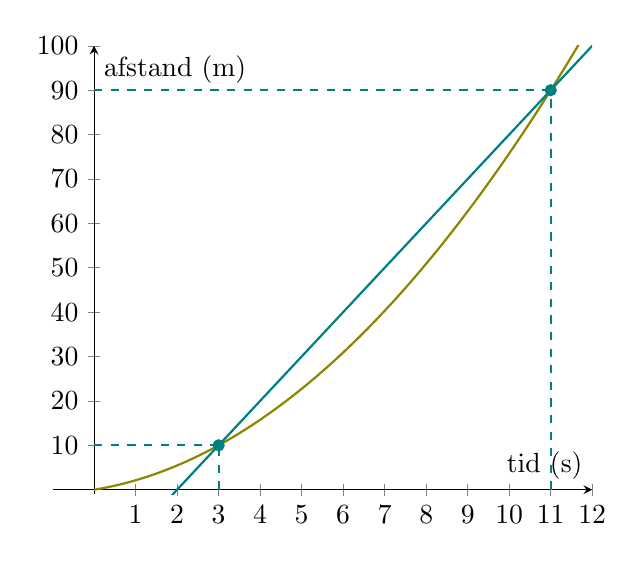
\begin{tikzpicture}
		\begin{axis}[
		axis lines = center, 
		xmin = -1, xmax = 12,
		ymin = -1, ymax = 100,
		xlabel = tid (s), ylabel = afstand (m),
		xtick = {0,1,...,11,12},
		ytick = {0,10,...,90,100},		]
			\addplot[color = olive, thick, domain = 0:12, samples = 300] {0.606*x^2+1.515*x};
			\filldraw[color = teal] (axis cs: 3,10) circle (2pt);
			\filldraw[color = teal] (axis cs: 11,90) circle (2pt);
			\addplot[color = teal, thick, domain = 0:12] {10*x-20}; 
			\draw[color = teal, dashed, thick] (axis cs: 3,0) -- (axis cs:3, 10);
			\draw[color = teal, dashed, thick] (axis cs: 0,10) -- (axis cs:3, 10);
			\draw[color = teal, dashed, thick] (axis cs: 11,0) -- (axis cs:11, 90);
			\draw[color = teal, dashed, thick] (axis cs: 0,90) -- (axis cs:11, 90);
		\end{axis}
		\end{tikzpicture}
		\caption{Afstandsfunktion samt sekant mellem punkterne.}
		\label{fig:sekant}
	\end{figure}
	Vi har fundet den gennemsnitlige hastighed fra 10 til 90 meter som hældningen af sekanten, altså 
	$a_s = 10$. Bilen accelererer dog, og derfor vil vi også forvente, at den korrekte hastighed efter 10 meter 
	vil være væsentligt lavere. Skal vi have et bedre bud på den korrekte hastighed, må vi altså skulle 
	rykke punktet $(t_1,y_1)$ tættere på $(t_0,y_0)$. Se for eksempel Figur \ref{fig:afstande}.
	\begin{figure}[H]
		\centering	
		\begin{tikzpicture}
		\newcommand{\sticky}[1]{
			\begin{tikzpicture}[scale = #1]
				\draw[color = teal,thick] (0,0) -- (1,2);
				\draw[color = teal,thick] (1,2) -- (2,0);
				\draw[color = teal,thick] (1,2) -- (1,4);
				\draw[color = teal,thick] (0,2.5) -- (1,4);
				\draw[color = teal, thick] (2,2.5) -- (1,4);
				\draw[color = teal, thick] (1,4.5) circle (0.5);
				\filldraw[color = teal]  (0,0) circle (0.1mm);
				\filldraw[color = teal]  (2,0) circle (0.1mm);
				\filldraw[color = teal]  (0,2.5) circle (0.1mm);
				\filldraw[color = teal]  (2,2.5) circle (0.1mm);
			\end{tikzpicture}		
		}
		\newcommand{\car}[1]{
			\begin{tikzpicture}[scale = #1]
				\draw[color = teal,thick] (0.5,0) -- (0.5,1);
				\draw[color = teal,thick] (0.5,1) -- (1,1);
				\draw[color = teal,thick] (1,1) -- (2,2);
				\draw[color = teal,thick] (2,2) -- (4,2);
				\draw[color = teal,thick] (4,2) -- (5,1);
				\draw[color = teal,thick] (5,1) -- (6,1);
				\draw[color = teal,thick] (6,1) -- (6,0);
				\draw[color = teal,thick] (1,1) -- (5,1);
				\draw[color = teal,thick] (3,2) -- (3,1);
				\draw[color = teal,thick] (0.5,0) -- (0.7,0);
				\draw[color = teal,thick] (1.5,0) circle (0.45);
				\draw[color = teal,thick] (2.3,0) -- (4.3,0);
				\draw[color = teal,thick] (5,0) circle (0.45);
				\draw[color = teal,thick] (5.8,0) -- (6,0);
				\draw[color = teal,thick] (3.7,1.4) circle (0.25);
			\end{tikzpicture}		
		}
		%First line
		\node[inner sep = 0mm] at (-2,0) (-1) {\phantom{\sticky{0.1}}};
		\node[inner sep = 0mm] at (0,0) (1) {\sticky{0.1}};
		\node[inner sep = 0mm] at (10,0) (2) {\sticky{0.1}};
		\draw[color = teal, thick] (-1.south west) -- (2.south east);
		\node[color = teal, below = 3mm] at (1) {10m};
		\node[color = teal, below = 3mm] at (2) {90m};
		\node[color = teal, below = 3mm] at (-1) {0m};
		\node[color = teal, above = 3mm] at (1) {3s};
		\node[color = teal, above = 3mm] at (2) {11s};
		\node[color = teal, above = 3mm] at (-1) {0s};
		\node[] at (5,0) {\car{0.2}};
		%Second line
		\node[inner sep = 0mm] at (-2,-2) (-1) {\phantom{\sticky{0.1}}};
		\node[inner sep = 0mm] at (0,-2) (1) {\sticky{0.1}};
		\node[inner sep = 0mm] at (6,-2) (2) {\sticky{0.1}};
		\draw[color = teal, thick] (-1.south west) -- (2.south east);
		\node[color = teal, below = 3mm] at (1) {10m};
		\node[color = teal, below = 3mm] at (2) {60m};
		\node[color = teal, below = 3mm] at (-1) {0m};
		\node[color = teal, above = 3mm] at (1) {3s};
		\node[color = teal, above = 3mm] at (2) {8.78s};
		\node[color = teal, above = 3mm] at (-1) {0s};
		\node[] at (3,-2) {\car{0.2}};
		%Third line
		\node[inner sep = 0mm] at (-2,-4) (-1) {\phantom{\sticky{0.1}}};
		\node[inner sep = 0mm] at (0,-4) (1) {\sticky{0.1}};
		\node[inner sep = 0mm] at (4,-4) (2) {\sticky{0.1}};
		\draw[color = teal, thick] (-1.south west) -- (2.south east);
		\node[color = teal, below = 3mm] at (1) {10m};
		\node[color = teal, below = 3mm] at (2) {40m};
		\node[color = teal, below = 3mm] at (-1) {0m};
		\node[color = teal, above = 3mm] at (1) {3s};
		\node[color = teal, above = 3mm] at (2) {6.97s};
		\node[color = teal, above = 3mm] at (-1) {0s};
		\node[] at (2,-4) {\car{0.2}};
		%Fourth line
		\node[inner sep = 0mm] at (-2,-6) (-1) {\phantom{\sticky{0.1}}};
		\node[inner sep = 0mm] at (0,-6) (1) {\sticky{0.1}};
		\node[inner sep = 0mm] at (3,-6) (2) {\sticky{0.1}};
		\draw[color = teal, thick] (-1.south west) -- (2.south east);
		\node[color = teal, below = 3mm] at (1) {10m};
		\node[color = teal, below = 3mm] at (2) {20m};
		\node[color = teal, below = 3mm] at (-1) {0m};
		\node[color = teal, above = 3mm] at (1) {3s};
		\node[color = teal, above = 3mm] at (2) {4.63s};
		\node[color = teal, above = 3mm] at (-1) {0s};
		\node[] at (1.5,-6) {\car{0.2}};
		\end{tikzpicture}
		\caption{Tider for tilbagelægning af afstande ved forskellige afstande fra $y_0$.}
		\label{fig:afstande}
	\end{figure}
	Vi kan ved de forskellige afstande bestemme den gennemsnitlige hastighed. På Tabel \ref{tab:gns} fremgår 
	gennemsnitshastighederne ved de forskellige målte afstande. 
	\begin{table}[H]
		\centering		
		\rowcolors{1}{teal!20}{white}		
		\begin{tabular}{ccccc}
			$y_1$ & 90m & 60m & 40m & 20m \\
			$t_1$ & 11s & 8.78s & 6.97s & 4.64s \\
			Fart  & 10$\frac{\textnormal{m}}{\textnormal{s}}$ & 8.65$\frac{\textnormal{m}}{\textnormal{s}}$
			& 7.56$\frac{\textnormal{m}}{\textnormal{s}}$ & 6.09$\frac{\textnormal{m}}{\textnormal{s}}$
		\end{tabular}
		\caption{Gennemsnitsfart for bilen over de forskellige afstande.}
		\label{tab:gns}
	\end{table}
	Hvis bilen accelererer på nogenlunde jævn vis, så må de gælde, at jo tættere punkterne $y_1$ og $y_0$ er på 
	hinanden, jo bedre et bud er sekanthældningen mellem punkterne på den korrekte hastighed i $(t_0,y_0)$. Vi 
	kan prøve at tegne sekanterne for hvert af punktparrende. Dette kan ses på Figur \ref{fig:sekanter}.
	\begin{figure}[H]
		\centering
		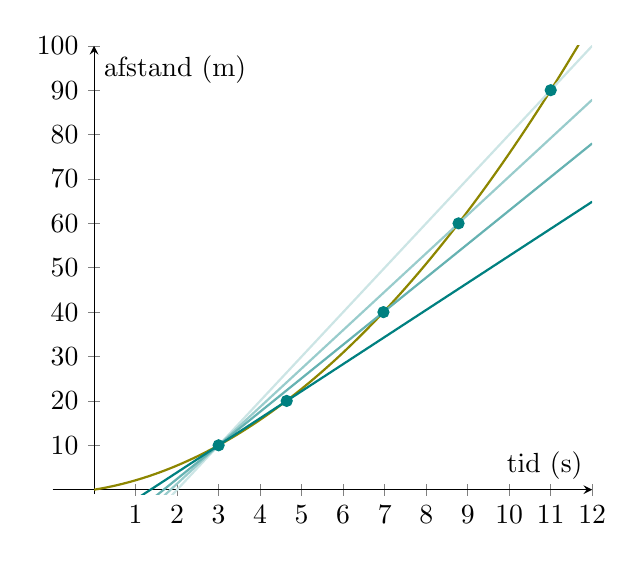
\begin{tikzpicture}
		\begin{axis}[
		axis lines = center, 
		xmin = -1, xmax = 12,
		ymin = -1, ymax = 100,
		xlabel = tid (s), ylabel = afstand (m),
		xtick = {0,1,...,11,12},
		ytick = {0,10,...,90,100},		]
			\addplot[color = olive, thick, domain = 0:12, samples = 300] {0.606*x^2+1.515*x};
			\addplot[color = teal!20, thick, domain = 0:12] {10*x-20}; 
			\addplot[color = teal!40, thick, domain = 0:12] {8.651*x-15.952}; 
			\addplot[color = teal!60, thick, domain = 0:12] {7.557*x-12.67}; 
			\addplot[color = teal, thick, domain = 0:12] {6.098*x-8.293}; 
			\filldraw[color = teal] (axis cs: 3,10) circle (2pt);
			\filldraw[color = teal] (axis cs: 11,90) circle (2pt);
			\filldraw[color = teal] (axis cs: 8.78,60) circle (2pt);
			\filldraw[color = teal] (axis cs: 6.97,40) circle (2pt);
			\filldraw[color = teal] (axis cs: 4.64,20) circle (2pt);
		\end{axis}
		\end{tikzpicture}
		\caption{Afstandsfunktionen med flere sekanter.}
		\label{fig:sekanter}
	\end{figure}
	Betragter vi Figur \ref{fig:sekanter}, kan vi se, at når punktet $(t_1,y_1)$ bevæger sig tættere og 
	tættere på $(t_0,y_0)$, så kommer vi nærmere og nærmere den korrekte hældning i punktet $(t_0,y_0)$, som jo
	netop er den hastighed, vi leder efter. 
\end{exa}

\section*{Tangenter}
\stepcounter{section}

Når vi lader et punkt bevæge sig mod et andet punkt, kan vi benytte os af grænseværdibegrebet. Først vil vi dog introducere \textit{tangentlinjer}.

\begin{defn}[Tangentlinje]
	Tangenten til grafen for en funktion $f$ i et punkt $x_0$ er en ret linje, der lokalt skærer grafen for $f$ 
	i kun et punkt $(x_0,f(x_0))$ og som følger langs grafen for $f$. 
\end{defn}
Der gælder for tangenten til en graf for en funktion $f$, at tangenten ligner grafen for $f$, når vi "zoomer" langt nok ind på grafen. 
\begin{exa}
	Vi vender nu tilbage til hastighedsmålingen af bilen. På Figur \ref{fig:sekanter} kunne vi se, hvordan 
	sekanternes hældning kom tættere og tættere på den korrekte hældning. Vi har nu på Figur \ref{fig:tangent}
	tilmed tegnet tangenten i punktet $(t_0,y_0)$ ind på grafen. 
	\begin{figure}[H]
		\centering
		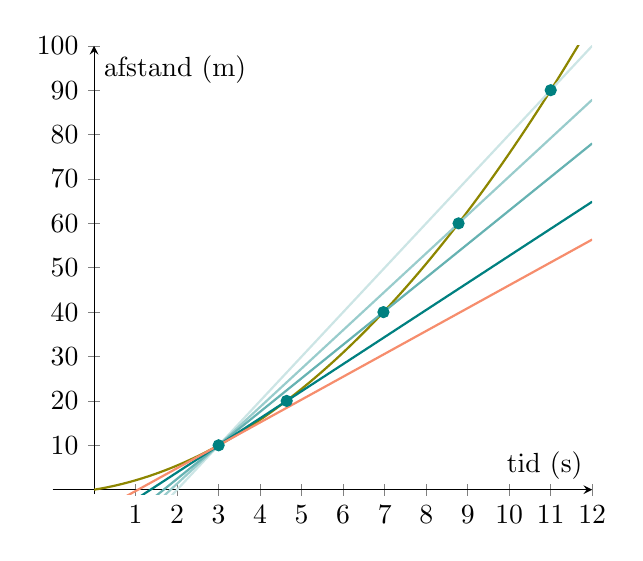
\begin{tikzpicture}
		\begin{axis}[
		axis lines = center, 
		xmin = -1, xmax = 12,
		ymin = -1, ymax = 100,
		xlabel = tid (s), ylabel = afstand (m),
		xtick = {0,1,...,11,12},
		ytick = {0,10,...,90,100},		]
			\addplot[color = olive, thick, domain = 0:12, samples = 300] {0.606*x^2+1.515*x};
			\addplot[color = teal!20, thick, domain = 0:12] {10*x-20}; 
			\addplot[color = teal!40, thick, domain = 0:12] {8.651*x-15.952}; 
			\addplot[color = teal!60, thick, domain = 0:12] {7.557*x-12.67}; 
			\addplot[color = teal, thick, domain = 0:12] {6.098*x-8.293}; 
			\addplot[color = Melon, thick, domain = 0:12] {5.151*x - 5.454}; 
			\filldraw[color = teal] (axis cs: 3,10) circle (2pt);
			\filldraw[color = teal] (axis cs: 11,90) circle (2pt);
			\filldraw[color = teal] (axis cs: 8.78,60) circle (2pt);
			\filldraw[color = teal] (axis cs: 6.97,40) circle (2pt);
			\filldraw[color = teal] (axis cs: 4.64,20) circle (2pt);
		\end{axis}
		\end{tikzpicture}
		\caption{Afstandsfunktionen med tangent.}
		\label{fig:tangent}
	\end{figure}
	Hældningen af tangenten må være den korrekte hastighed nøjagtigt i punktet $(t_0,y_0)$ og dermed den, vi 
	søger. 
\end{exa}

\section*{Differentialkvotienten}
\stepcounter{section}

Vi har set, hvordan vi kan bruge hældningen af sekantlinjer til at tilnærme hastigheder, og vi har set, hvordan
sekanter bevæger sig mod tangenter, når skæringspunkterne for sekantlinjen bevæger sig mod hinanden. Vi vil nu præcisere disse begreber yderligere. 

\begin{defn}[Differenskvotienten]
	For en funktion $f$ kaldes hældningen af sekanten $a_s$ igennem to punkter $(x_0,f(x_0))$ og 
	$(x_0+h,f(x_0 + h))$ for \textit{differenskvotienten}.
\end{defn}
En visualisering af dette fremgår af Figur \ref{fig:differenskvotient}.
\begin{figure}[H]
	\centering
	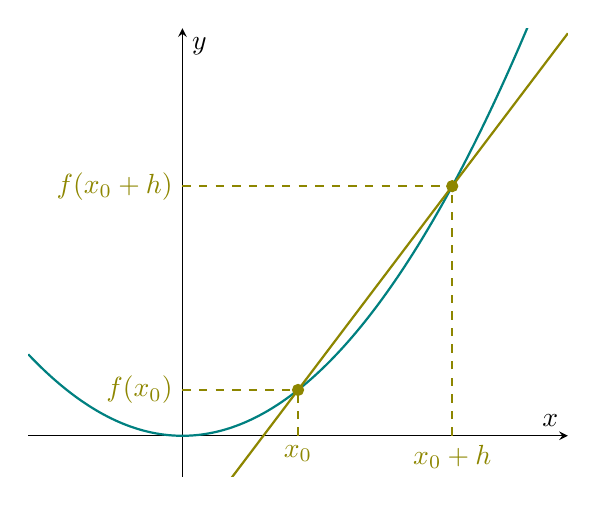
\begin{tikzpicture}
	\begin{axis}[
	axis lines = center, 
	xmin = -2, xmax = 5,
	ymin = -2, ymax = 20,
	xlabel = $x$, ylabel = $y$,
	ticks = none	]
		\addplot[color = teal, thick, domain = -2:5, samples = 200] {x^2}; 
		\draw[color = olive, dashed, thick] (axis cs: 1.5,0) -- (axis cs:1.5, 2.25);
		\draw[color = olive, dashed, thick] (axis cs: 0,2.25) -- (axis cs:1.5, 2.25);
		\draw[color = olive, dashed, thick] (axis cs: 3.5,0) -- (axis cs:3.5, 12.25);
		\draw[color = olive, dashed, thick] (axis cs: 0,12.25) -- (axis cs:3.5, 12.25);
		\addplot[color = olive, thick, domain = -1:5] {5*x-5.25};
		\filldraw[color = olive] (axis cs: 1.5,2.25) circle (2pt);
		\filldraw[color = olive] (axis cs: 3.5,12.25) circle (2pt);
		\node[color = olive, anchor = north] at (axis cs:1.5,0) {$x_0$};
		\node[color = olive, anchor = north] at (axis cs:3.5,0) {$x_0+h$};
		\node[color = olive, anchor = east] at (axis cs:0,2.25) {$f(x_0)$};
		\node[color = olive, anchor = east] at (axis cs:0,12.25) {$f(x_0+h)$};
	\end{axis}
	\end{tikzpicture}
	\caption{Differenskvotienten}
	\label{fig:differenskvotient}
\end{figure}
\begin{setn}[Differenskvotienten]
	Differenskvotienten eller sekanthældningen for $f$ er gennem $(x_0,f(x_0))$ og $(x_0+h,f(x_0+h))$ er 
	givet ved
	\begin{align*}
		a_s = \frac{f(x_0 + h) - f(x_0)}{h}.
	\end{align*}
\end{setn}
\begin{proof}
	Vi betragter Figur \ref{fig:differenskvotient} og husker os selv på, at hældningskoefficienten for en 
	ret linje er givet ved
	\begin{align*}
		a_s = \frac{y_2 - y_1}{x_2-x_1}.
	\end{align*}
	Vi indsætter nu funktionsværdierne og får
	\begin{align*}
		a_s = \frac{f(x_0 + h)-f(x_0)}{x_0 + h - x_0} = \frac{f(x_0 + h) - f(x_0)}{h}.
	\end{align*}
\end{proof}

Tanken er nu som følger: Hvis sekantlinjen går mod tangentlinjen i $x_0$, når $x_0 + h$ går mod $x_0$, så må vi have, at sekanthældningen går mod tangenthældningen, når $h$ bliver meget lille. Vi kan med dette bruge grænseværdibegrebet til at definere \textit{differentialkvotienten} i $x_0$. 
\begin{defn}[Differentialkvotienten]
	Differentialkvotienten for en funktion $f$ i et punkt $x_0$ defineres som grænseværdien
	\begin{align*}
		\lim_{h \to 0} \frac{f(x_0 + h)-f(x_0)}{h}
	\end{align*}
	af differenskvotienten i fald grænseværdien eksisterer. Vi betegner differentialkvotienten af $f$ i $x_0$ 
	ved
	\begin{align*}
		f'(x_0).
	\end{align*}
	Tilmed defineres funktionen $f'(x)$, der til ethvert punkt $x_0$ giver differentialkvotienten som den
	afledede af $f$. 
\end{defn}
Dette læses "f-mærke af $x_0$".

\newpage

\subsection*{Opgave 1}

Tegn i Geogebra funktionen $f(x) = x^2$. Sæt nu to punkter på linjen, $(1,f(1))$ og $(1+h,f(1+h))$. Geogebra vil så oprette en skyder til dig. Tegn sekanten gennem disse to punkter. Hvad sker der med sekanthældningen, når vi lader $h$ gå mod $0$? Gør det samme for følgende punkter og udfyld tabellen

\begin{center}
	\begin{tabular}{c|p{0.5cm}| >{\centering\arraybackslash} p{0.5cm}|>{\centering\arraybackslash} p{0.5cm}
	| >{\centering\arraybackslash} p{0.5cm}| >{\centering\arraybackslash} p{0.5cm}
	| >{\centering\arraybackslash} p{0.5cm}|>{\centering\arraybackslash} p{0.5cm}}
		$x_0$ & $-3$ & $-2$ & $-1$ & $0$ & 1 & 2 & 3 \\
		\hline
		Tangenthældning & & & & & & &
	\end{tabular}
\end{center}

Kan du gennemskue et mønster? Kan vi finde en funktion, der kan give os tangenthældningen for $f$ i et punkt
$x_0$?

\subsection*{Opgave 2}

Gør det samme som i Opgave 1, men nu med følgende funktioner
\begin{enumerate}[label=\roman*)]
	\item $f(x) = x^2 + 5$
	\item $f(x) = 2x^2$
	\item $f(x) = 5x^2$
	\item $f(x) = x^3$
\end{enumerate}

Hvad sker der med tangenthældningen for en funktion, hvis vi lægger en konstant til en funktion? Hvad sker der med tangenthældningen, hvis vi ganger en funktion med en konstant?

\subsection*{Opgave 3}

Gør det samme som i Opgave 1 for funktionen
\begin{align*}
	g(x) = 
	\begin{cases}
		-x^3 - 9, &\textnormal{ hvis } x < -2,\\
		-3x^2- 5x + 1, &\textnormal{ hvis } x \geq -2. 
	\end{cases}
\end{align*}
i punktet $(-2,g(-2))$. Hvad bliver tangenthældningen, når vi lader $h$ gå mod 0 fra højre. Hvad med fra venstre? Er tangenthældningen defineret i dette punkt?
